% Auto-generated figure index for hw-1 paper
% Generated by paper_figures/generate_all.py

% Figure 1: Version evolution timeline showing design iterations from V01 to V24.
\begin{figure}[htbp]
  \centering
  \includegraphics[width=\textwidth]{pdf/fig1_version_evolution.pdf}
  \caption{Version evolution timeline showing design iterations from V01 to V24.}
  \label{fig:1}
\end{figure}

% Figure 2: Stability domain comparison across control strategies (V13-V16).
\begin{figure}[htbp]
  \centering
  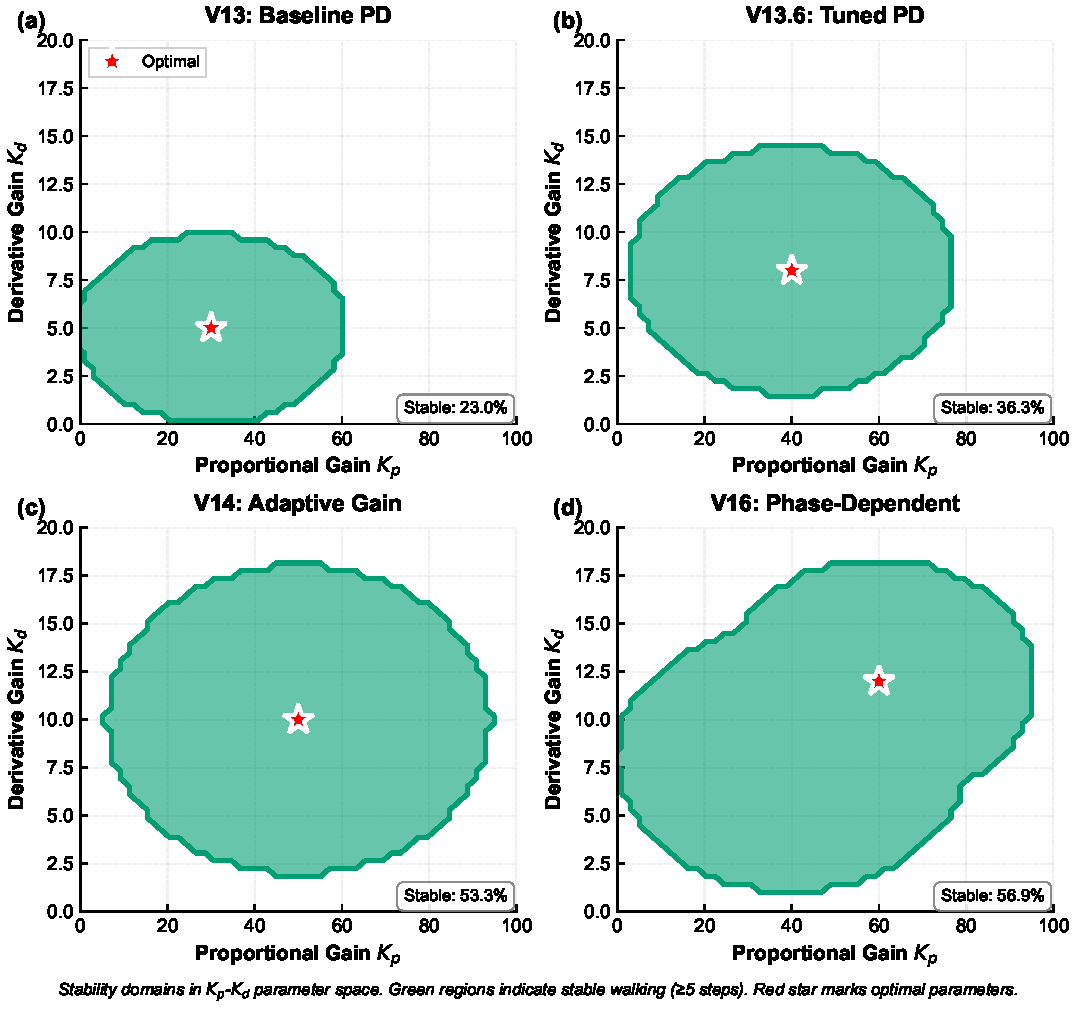
\includegraphics[width=\textwidth]{pdf/fig2_stability_domain.pdf}
  \caption{Stability domain comparison across control strategies (V13-V16).}
  \label{fig:2}
\end{figure}

% Figure 3: Energy analysis and cost of transport comparison.
\begin{figure}[htbp]
  \centering
  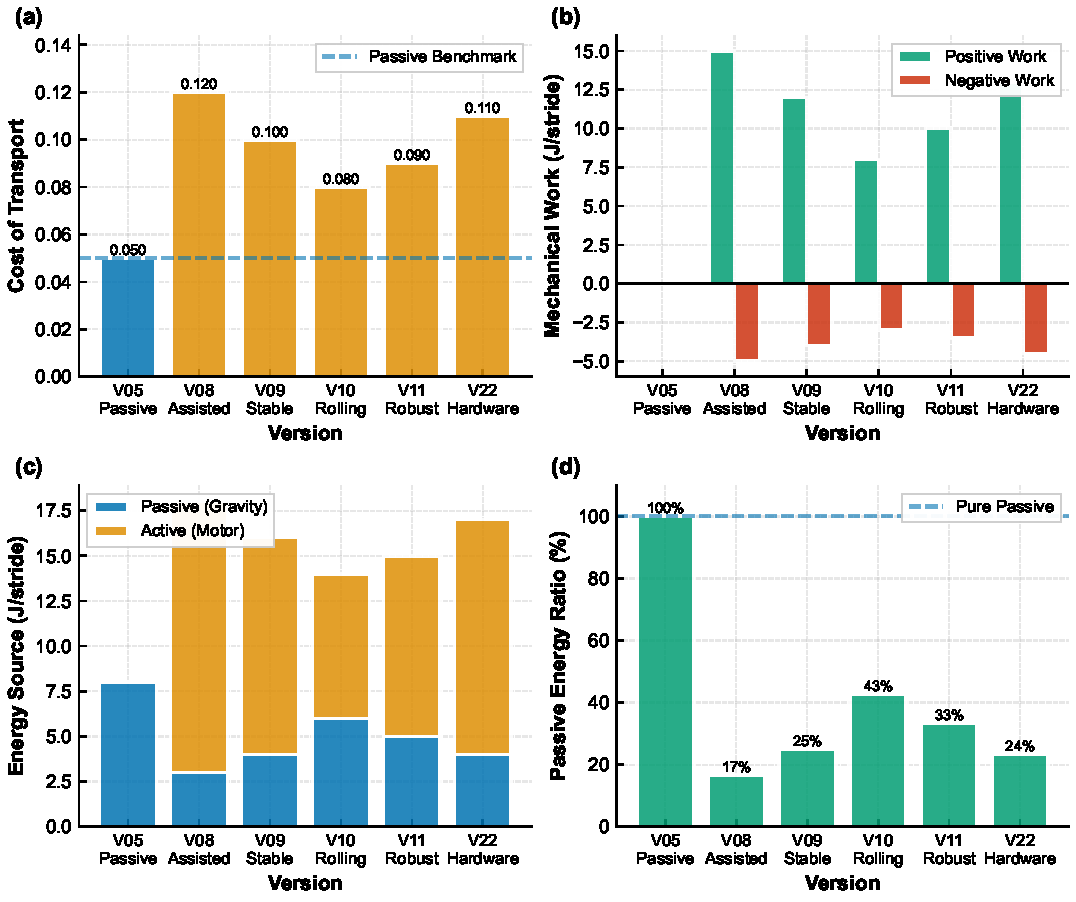
\includegraphics[width=\textwidth]{pdf/fig3_energy_analysis.pdf}
  \caption{Energy analysis and cost of transport comparison.}
  \label{fig:3}
\end{figure}

% Figure 4: Phase portrait, limit cycle, and basin of attraction.
\begin{figure}[htbp]
  \centering
  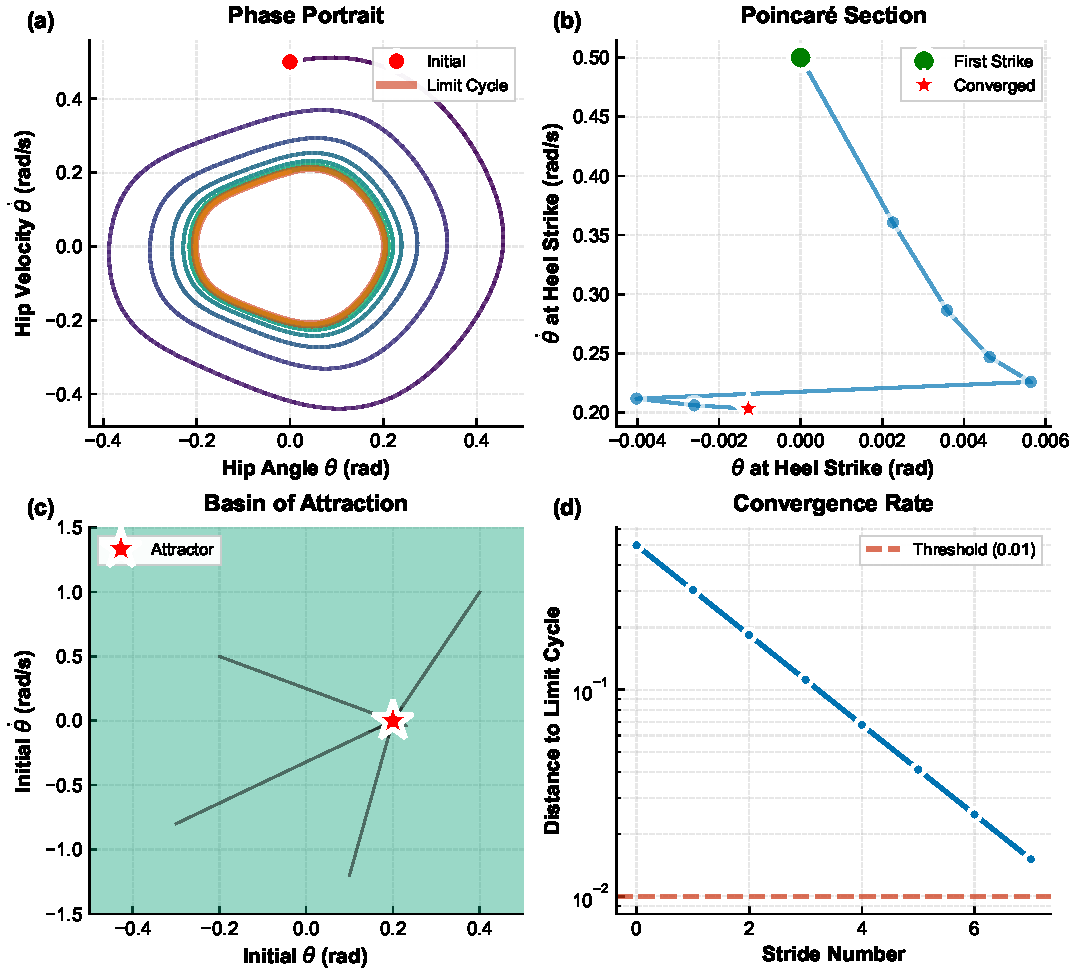
\includegraphics[width=\textwidth]{pdf/fig4_phase_portrait.pdf}
  \caption{Phase portrait, limit cycle, and basin of attraction.}
  \label{fig:4}
\end{figure}

% Figure 5: Hardware specifications and mechanical design of V22 prototype.
\begin{figure}[htbp]
  \centering
  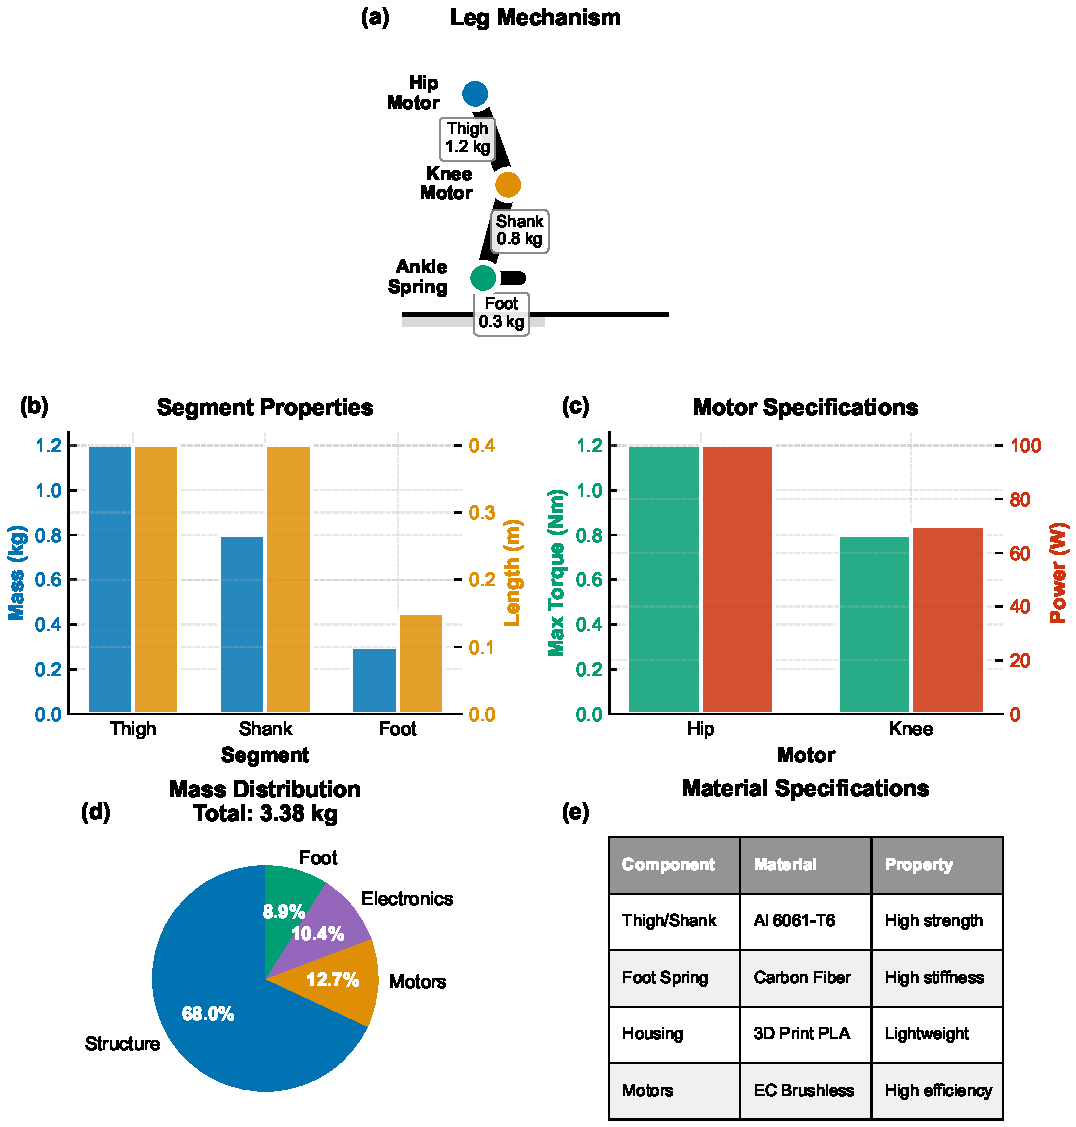
\includegraphics[width=\textwidth]{pdf/fig5_hardware_specs.pdf}
  \caption{Hardware specifications and mechanical design of V22 prototype.}
  \label{fig:5}
\end{figure}

% Usage:
%   % Auto-generated figure index for hw-1 paper
% Generated by paper_figures/generate_all.py

% Figure 1: Version evolution timeline showing design iterations from V01 to V24.
\begin{figure}[htbp]
  \centering
  \includegraphics[width=\textwidth]{pdf/fig1_version_evolution.pdf}
  \caption{Version evolution timeline showing design iterations from V01 to V24.}
  \label{fig:1}
\end{figure}

% Figure 2: Stability domain comparison across control strategies (V13-V16).
\begin{figure}[htbp]
  \centering
  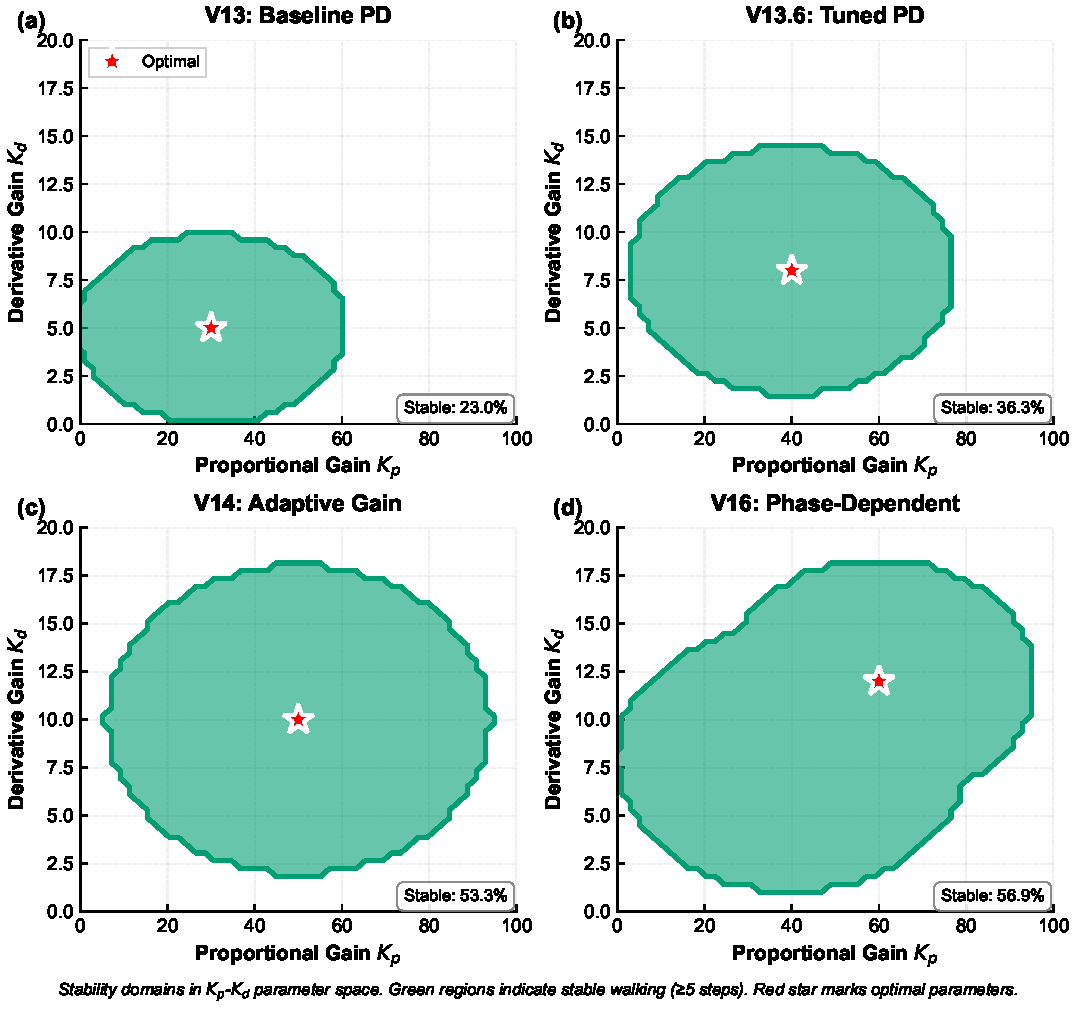
\includegraphics[width=\textwidth]{pdf/fig2_stability_domain.pdf}
  \caption{Stability domain comparison across control strategies (V13-V16).}
  \label{fig:2}
\end{figure}

% Figure 3: Energy analysis and cost of transport comparison.
\begin{figure}[htbp]
  \centering
  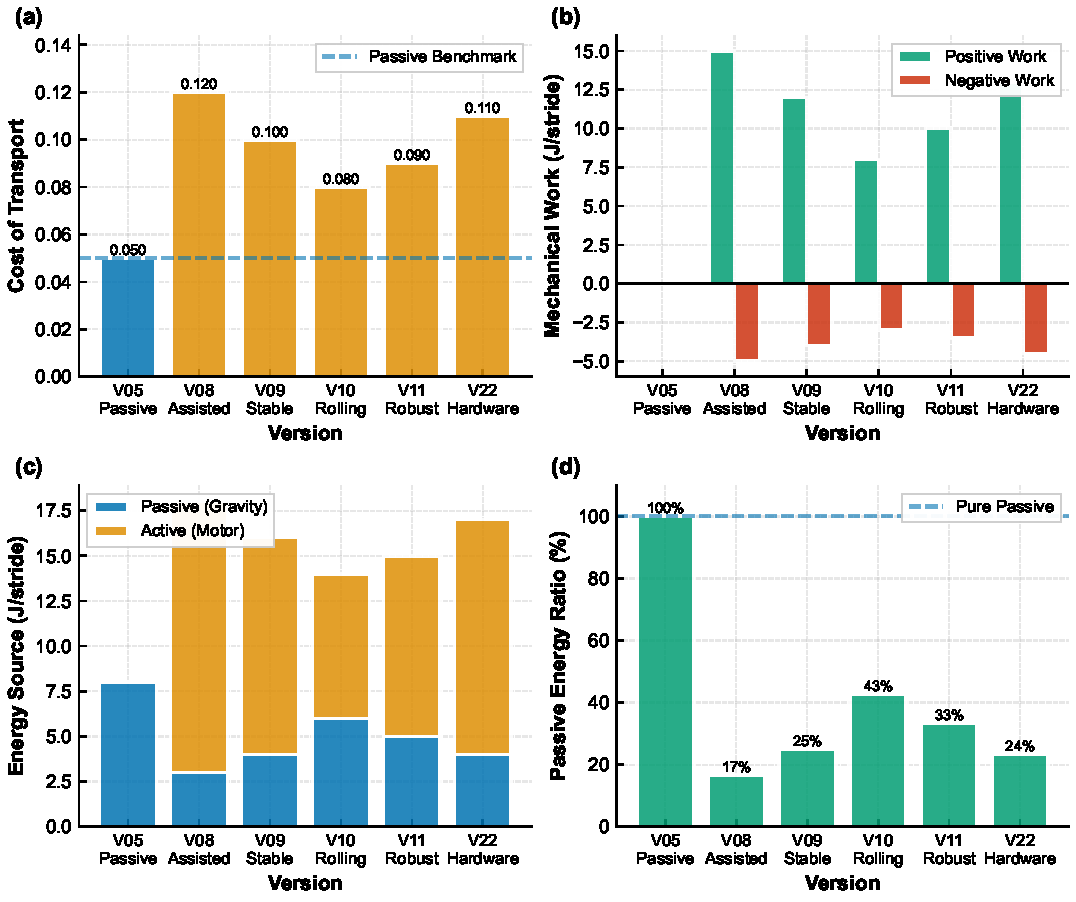
\includegraphics[width=\textwidth]{pdf/fig3_energy_analysis.pdf}
  \caption{Energy analysis and cost of transport comparison.}
  \label{fig:3}
\end{figure}

% Figure 4: Phase portrait, limit cycle, and basin of attraction.
\begin{figure}[htbp]
  \centering
  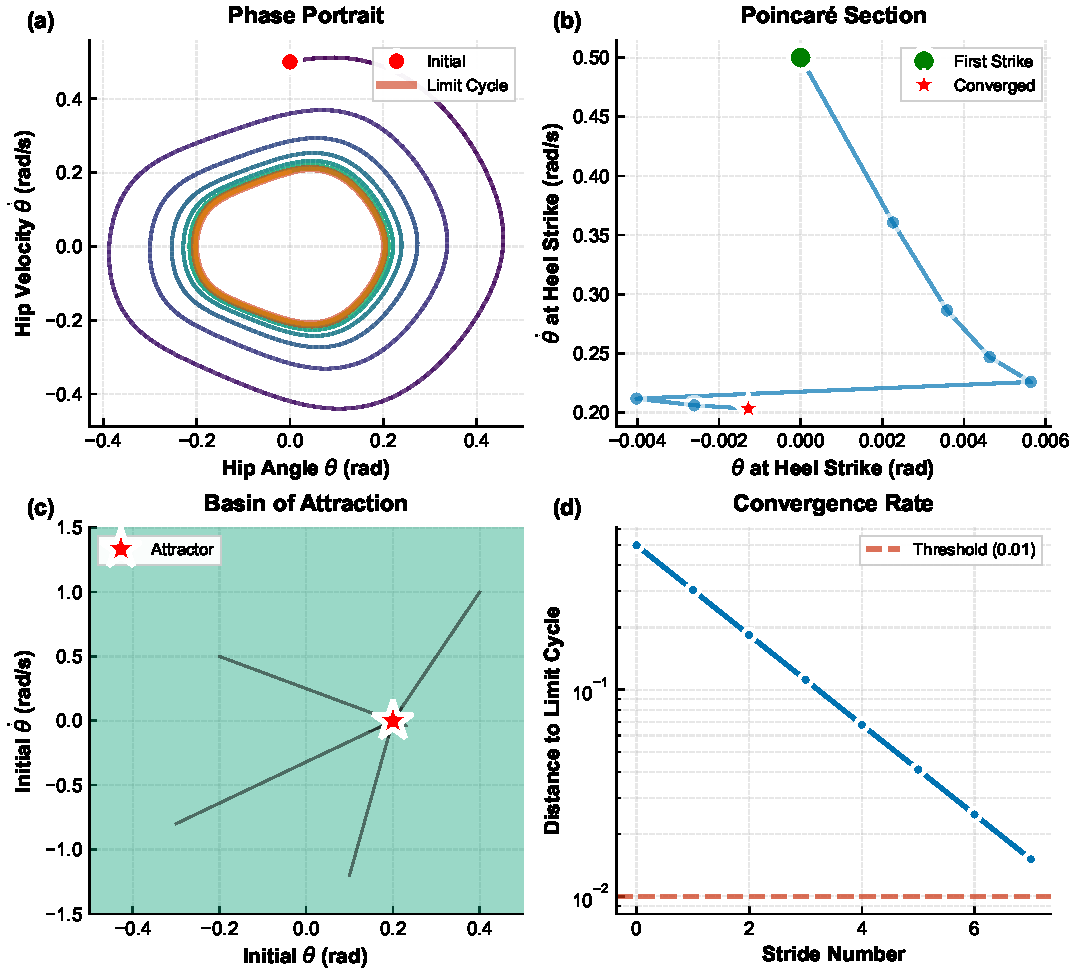
\includegraphics[width=\textwidth]{pdf/fig4_phase_portrait.pdf}
  \caption{Phase portrait, limit cycle, and basin of attraction.}
  \label{fig:4}
\end{figure}

% Figure 5: Hardware specifications and mechanical design of V22 prototype.
\begin{figure}[htbp]
  \centering
  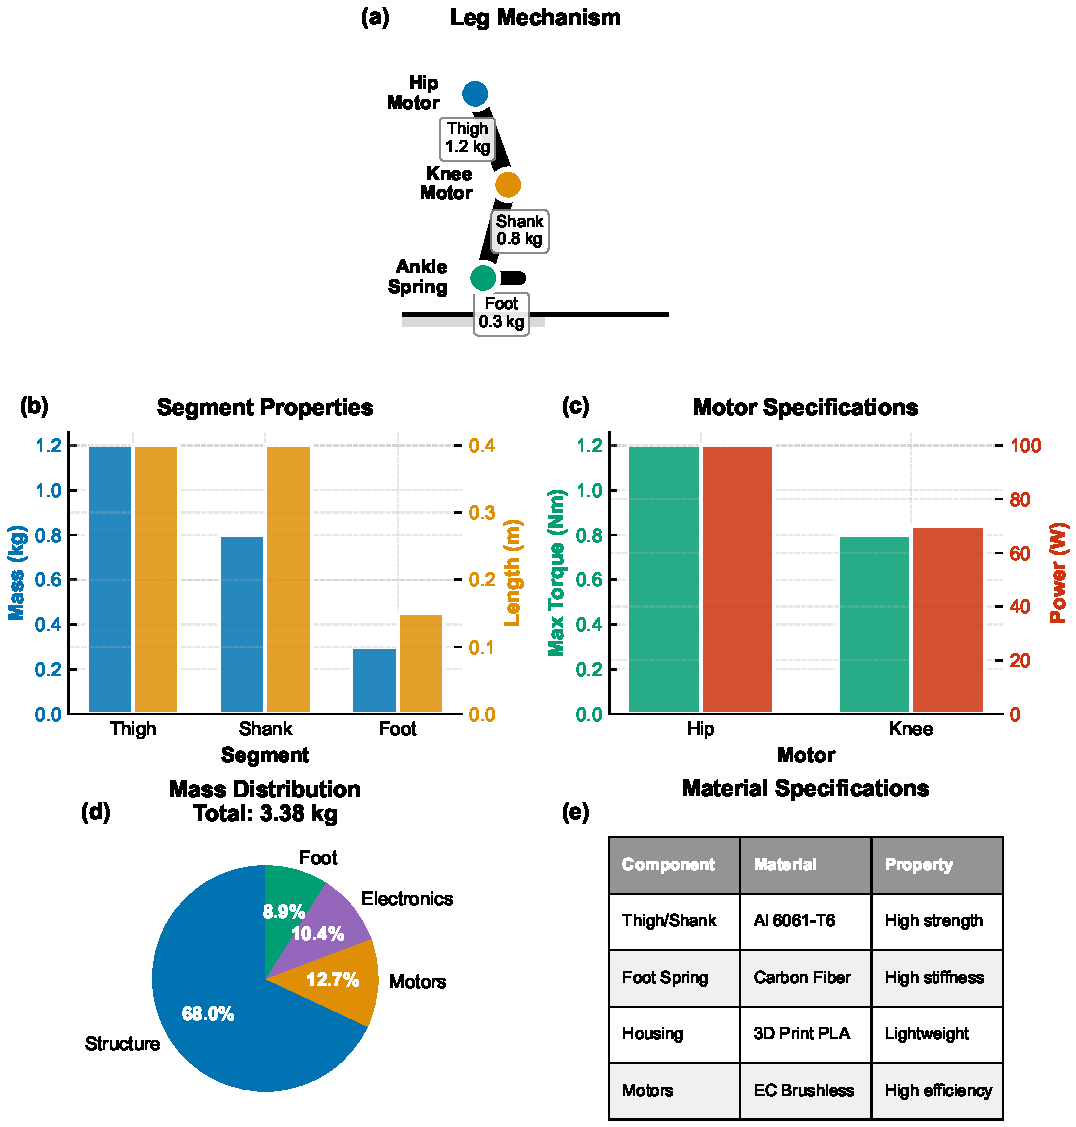
\includegraphics[width=\textwidth]{pdf/fig5_hardware_specs.pdf}
  \caption{Hardware specifications and mechanical design of V22 prototype.}
  \label{fig:5}
\end{figure}

% Usage:
%   % Auto-generated figure index for hw-1 paper
% Generated by paper_figures/generate_all.py

% Figure 1: Version evolution timeline showing design iterations from V01 to V24.
\begin{figure}[htbp]
  \centering
  \includegraphics[width=\textwidth]{pdf/fig1_version_evolution.pdf}
  \caption{Version evolution timeline showing design iterations from V01 to V24.}
  \label{fig:1}
\end{figure}

% Figure 2: Stability domain comparison across control strategies (V13-V16).
\begin{figure}[htbp]
  \centering
  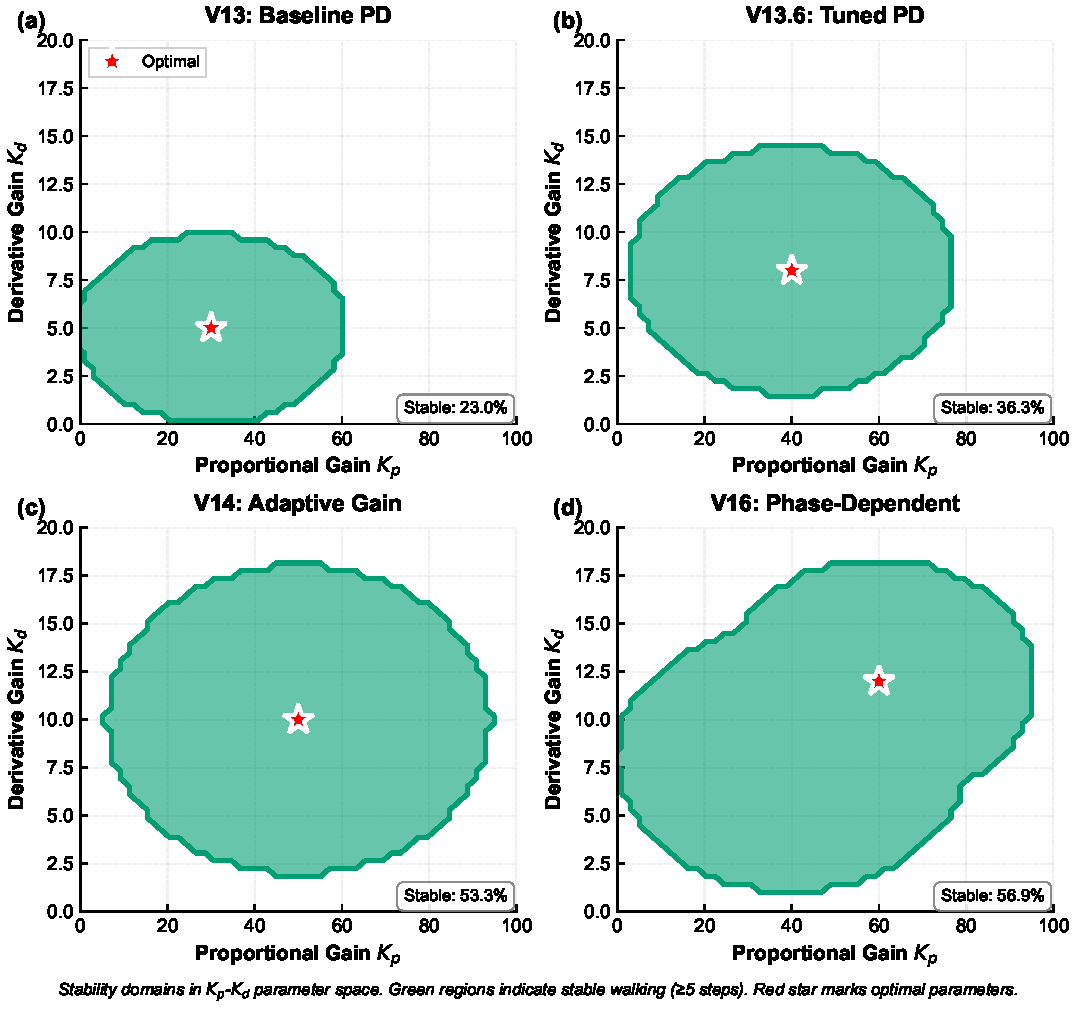
\includegraphics[width=\textwidth]{pdf/fig2_stability_domain.pdf}
  \caption{Stability domain comparison across control strategies (V13-V16).}
  \label{fig:2}
\end{figure}

% Figure 3: Energy analysis and cost of transport comparison.
\begin{figure}[htbp]
  \centering
  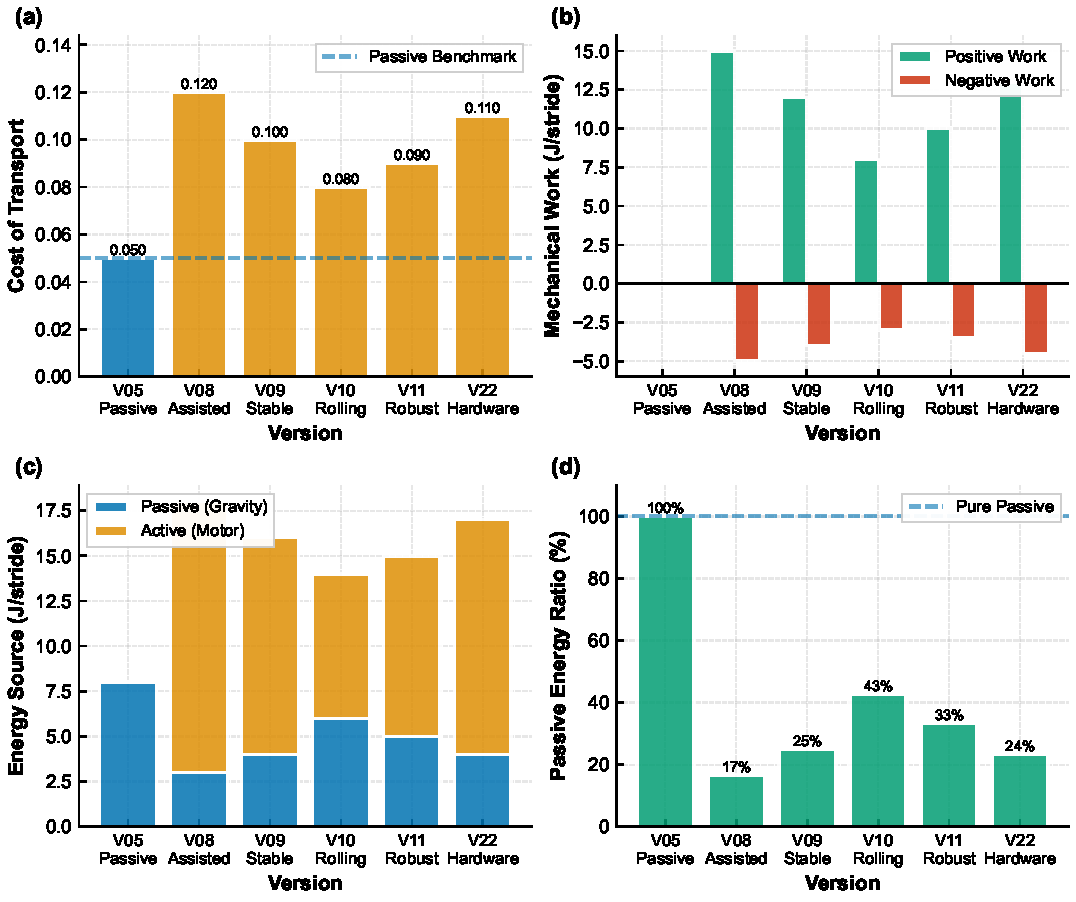
\includegraphics[width=\textwidth]{pdf/fig3_energy_analysis.pdf}
  \caption{Energy analysis and cost of transport comparison.}
  \label{fig:3}
\end{figure}

% Figure 4: Phase portrait, limit cycle, and basin of attraction.
\begin{figure}[htbp]
  \centering
  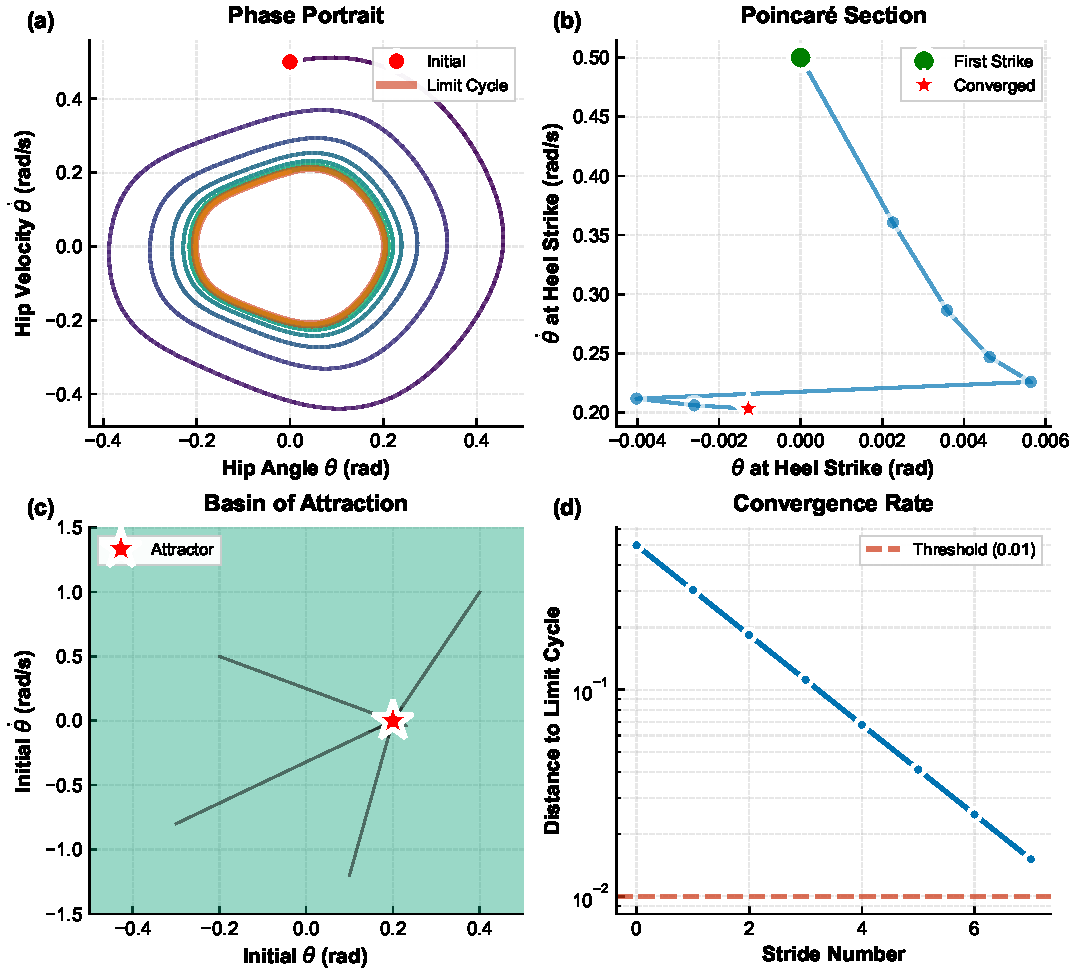
\includegraphics[width=\textwidth]{pdf/fig4_phase_portrait.pdf}
  \caption{Phase portrait, limit cycle, and basin of attraction.}
  \label{fig:4}
\end{figure}

% Figure 5: Hardware specifications and mechanical design of V22 prototype.
\begin{figure}[htbp]
  \centering
  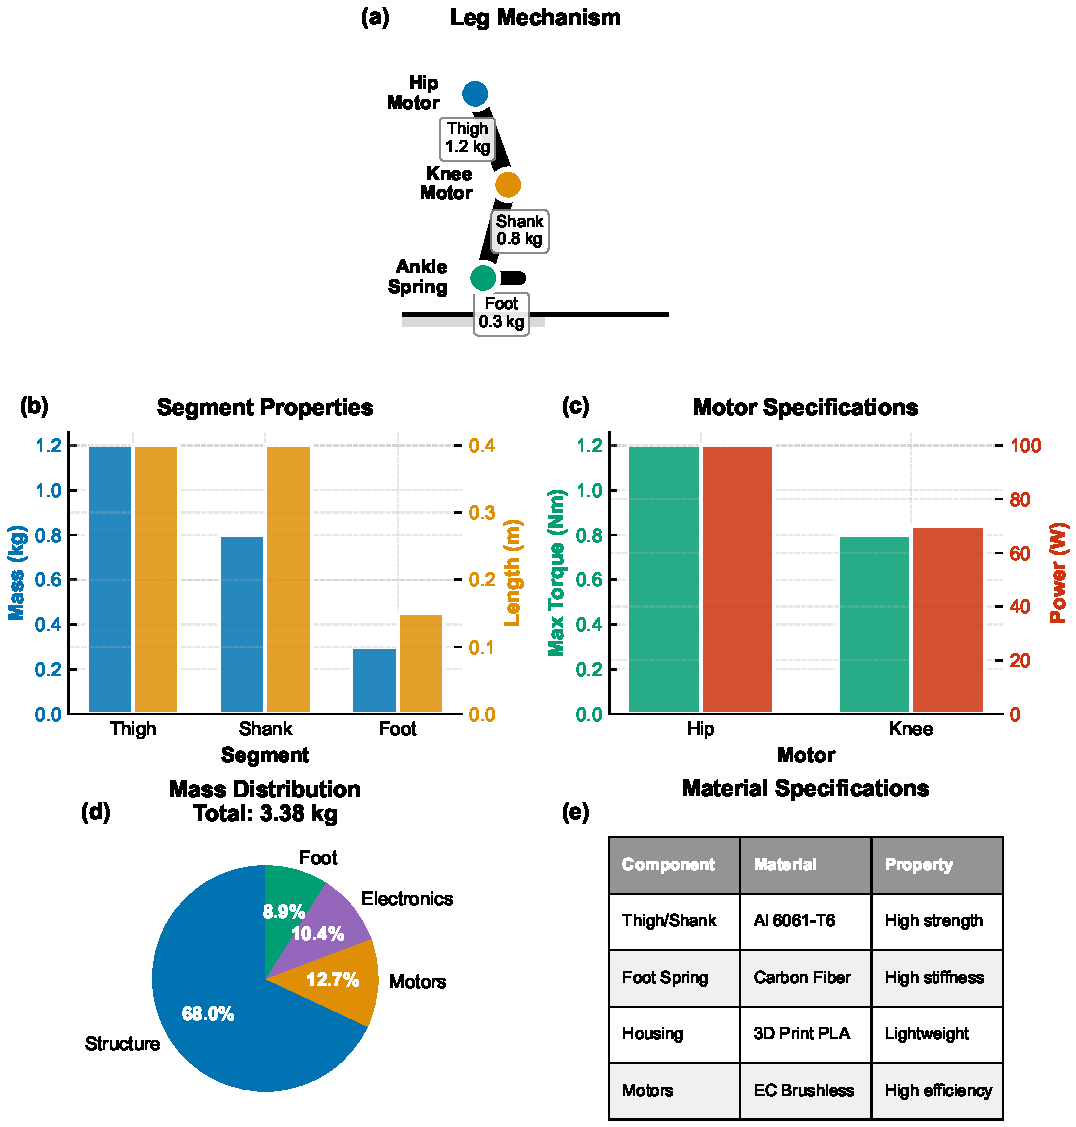
\includegraphics[width=\textwidth]{pdf/fig5_hardware_specs.pdf}
  \caption{Hardware specifications and mechanical design of V22 prototype.}
  \label{fig:5}
\end{figure}

% Usage:
%   % Auto-generated figure index for hw-1 paper
% Generated by paper_figures/generate_all.py

% Figure 1: Version evolution timeline showing design iterations from V01 to V24.
\begin{figure}[htbp]
  \centering
  \includegraphics[width=\textwidth]{pdf/fig1_version_evolution.pdf}
  \caption{Version evolution timeline showing design iterations from V01 to V24.}
  \label{fig:1}
\end{figure}

% Figure 2: Stability domain comparison across control strategies (V13-V16).
\begin{figure}[htbp]
  \centering
  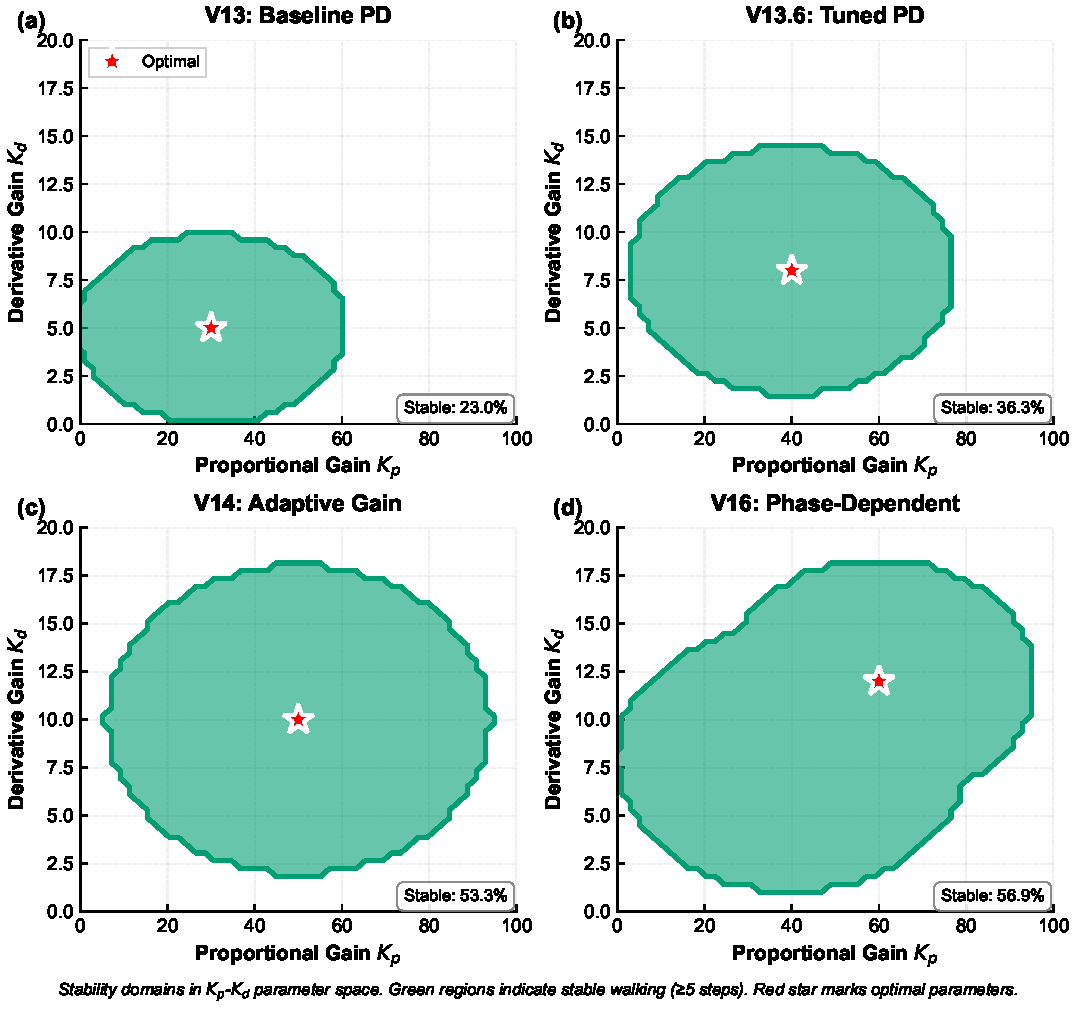
\includegraphics[width=\textwidth]{pdf/fig2_stability_domain.pdf}
  \caption{Stability domain comparison across control strategies (V13-V16).}
  \label{fig:2}
\end{figure}

% Figure 3: Energy analysis and cost of transport comparison.
\begin{figure}[htbp]
  \centering
  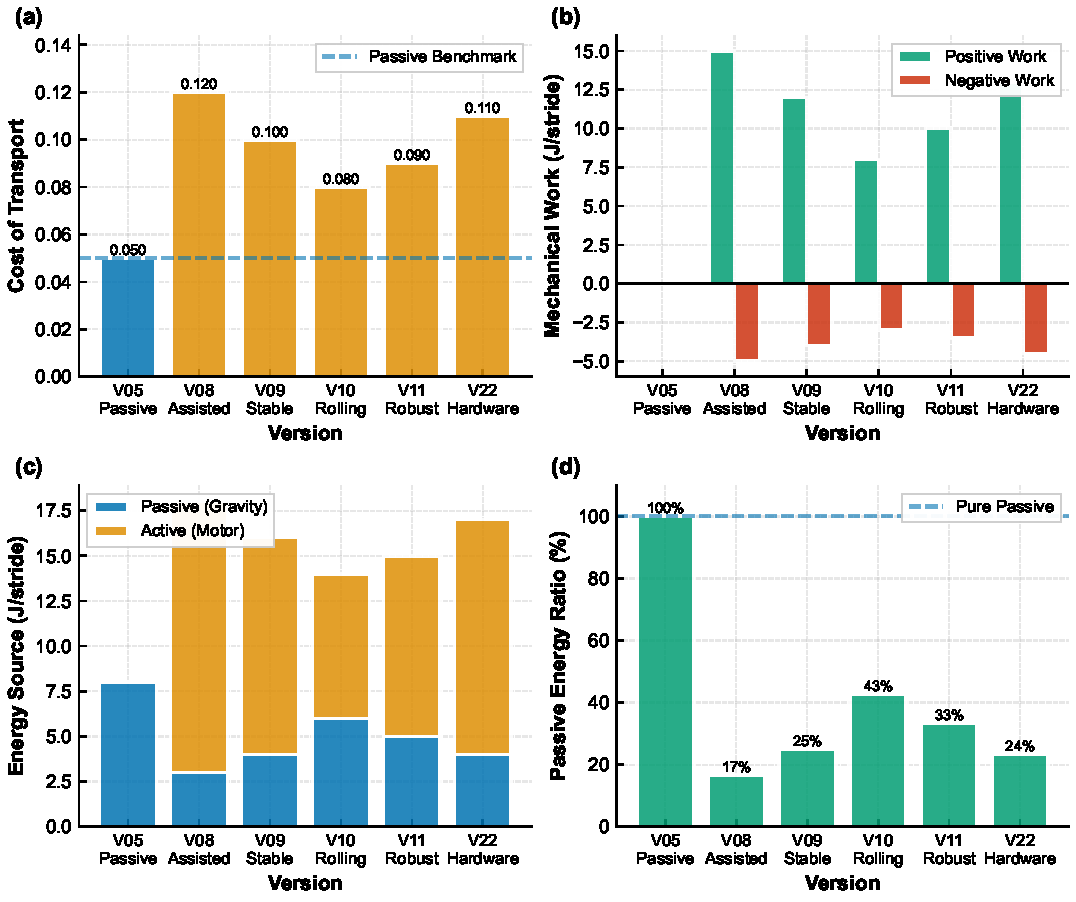
\includegraphics[width=\textwidth]{pdf/fig3_energy_analysis.pdf}
  \caption{Energy analysis and cost of transport comparison.}
  \label{fig:3}
\end{figure}

% Figure 4: Phase portrait, limit cycle, and basin of attraction.
\begin{figure}[htbp]
  \centering
  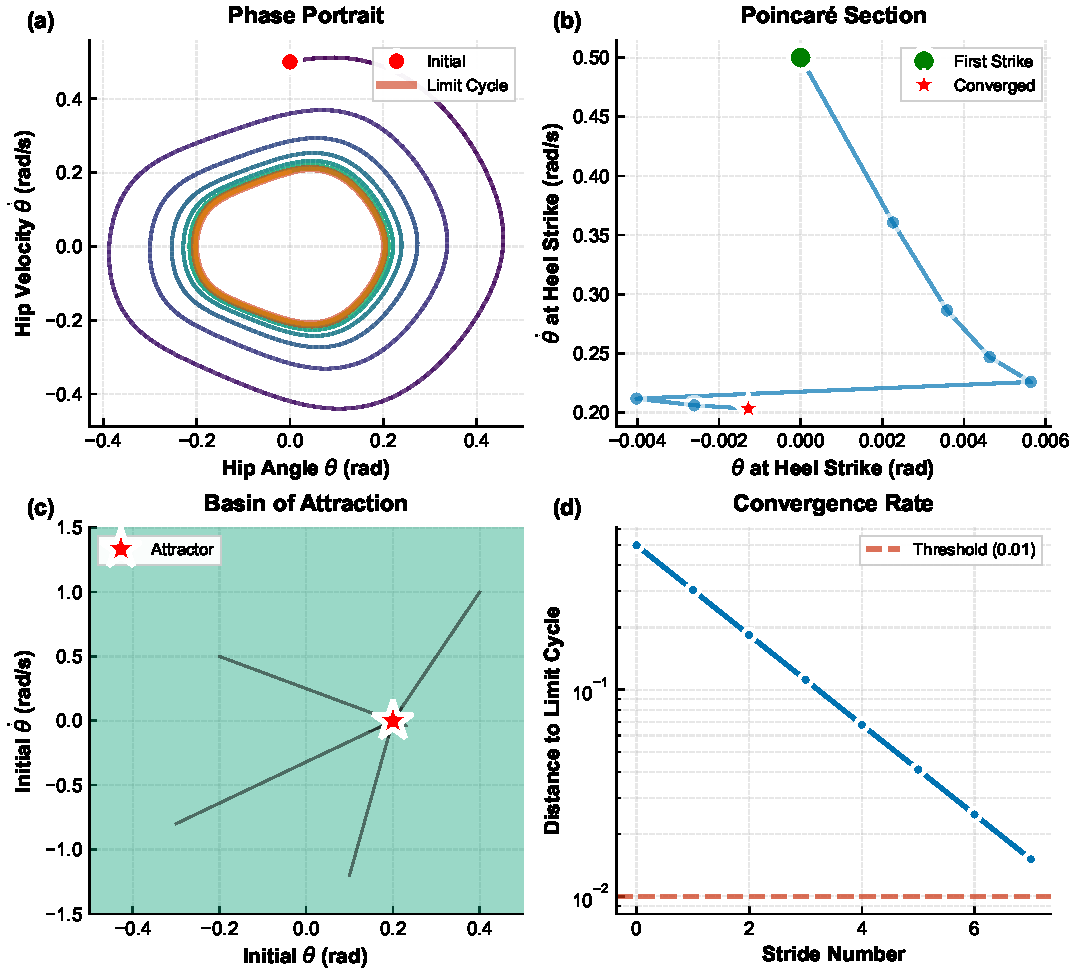
\includegraphics[width=\textwidth]{pdf/fig4_phase_portrait.pdf}
  \caption{Phase portrait, limit cycle, and basin of attraction.}
  \label{fig:4}
\end{figure}

% Figure 5: Hardware specifications and mechanical design of V22 prototype.
\begin{figure}[htbp]
  \centering
  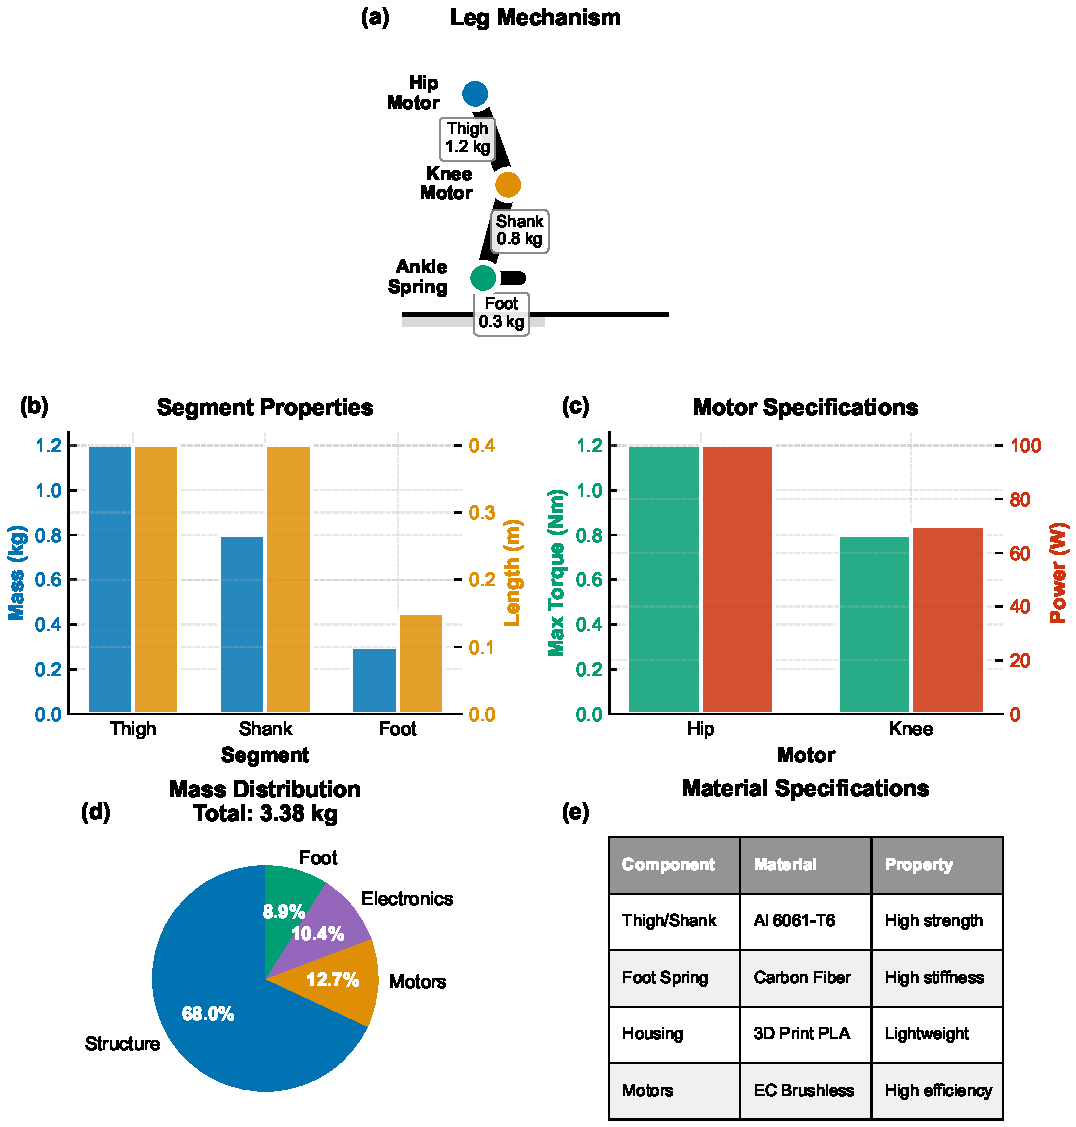
\includegraphics[width=\textwidth]{pdf/fig5_hardware_specs.pdf}
  \caption{Hardware specifications and mechanical design of V22 prototype.}
  \label{fig:5}
\end{figure}

% Usage:
%   \input{output/figures_index.tex}
%
% Or include individual figures:
%   \includegraphics[width=0.8\textwidth]{output/pdf/fig1_version_evolution.pdf}

%
% Or include individual figures:
%   \includegraphics[width=0.8\textwidth]{output/pdf/fig1_version_evolution.pdf}

%
% Or include individual figures:
%   \includegraphics[width=0.8\textwidth]{output/pdf/fig1_version_evolution.pdf}

%
% Or include individual figures:
%   \includegraphics[width=0.8\textwidth]{output/pdf/fig1_version_evolution.pdf}
